\chapter{\ifproject%
\ifenglish Project Structure and Methodology\else โครงสร้างและขั้นตอนการทำงาน\fi
\else%
\ifenglish Project Structure\else โครงสร้างของโครงงาน\fi
\fi
}

ในบทนี้จะกล่าวถึงหลักการ และการออกแบบระบบ

\makeatletter

% \renewcommand\section{\@startsection {section}{1}{\z@}%
%                                    {13.5ex \@plus -1ex \@minus -.2ex}%
%                                    {2.3ex \@plus.2ex}%
%                                    {\normalfont\large\bfseries}}

\makeatother
%\vspace{2ex}
% \titleformat{\section}{\normalfont\bfseries}{\thesection}{1em}{}
% \titlespacing*{\section}{0pt}{10ex}{0pt}

\section{โครงสร้างและขั้นตอนการพัฒนา}
\label{sec:development-structure}

\subsection{การวิจัยผู้ใช้และวิเคราะห์ปัญหา (User Research \& Problem Analysis)}
\label{subsec:user-research}

ในขั้นตอนนี้จะมุ่งเน้นการทำความเข้าใจผู้ใช้และปัญหาที่แท้จริงผ่านวิธีการต่างๆ เช่น
\begin{itemize}
    \item การสัมภาษณ์ผู้มีส่วนได้ส่วนเสีย (Stakeholder Interviews)
    \item การสังเกตการณ์และการศึกษาพฤติกรรมผู้ใช้ (User Observation \& Behavior Study)
    \item การวิเคราะห์คู่แข่งและตลาด (Competitor \& Market Analysis)
    \item การระบุ pain points และความต้องการที่แท้จริง (Pain Points \& Real Needs Identification)
\end{itemize}

\subsection{การกำหนดขอบเขตและข้อกำหนด (Scope \& Requirements Definition)}
\label{subsec:requirements-definition}

หลังจากเข้าใจปัญหาแล้ว ขั้นตอนนี้จะเป็นการกำหนดขอบเขตและข้อกำหนดที่ชัดเจน:
\begin{itemize}
    \item การระบุขอบเขตโซลูชัน (Solution Scope)
    \item การจัดลำดับความสำคัญของปัญหา (Problem Prioritization)
    \item การกำหนดข้อกำหนดซอฟต์แวร์ (Software Requirements)
    \item การสร้าง Problem-to-Feature Mapping
\end{itemize}

\begin{figure}[h!]
  \centering
  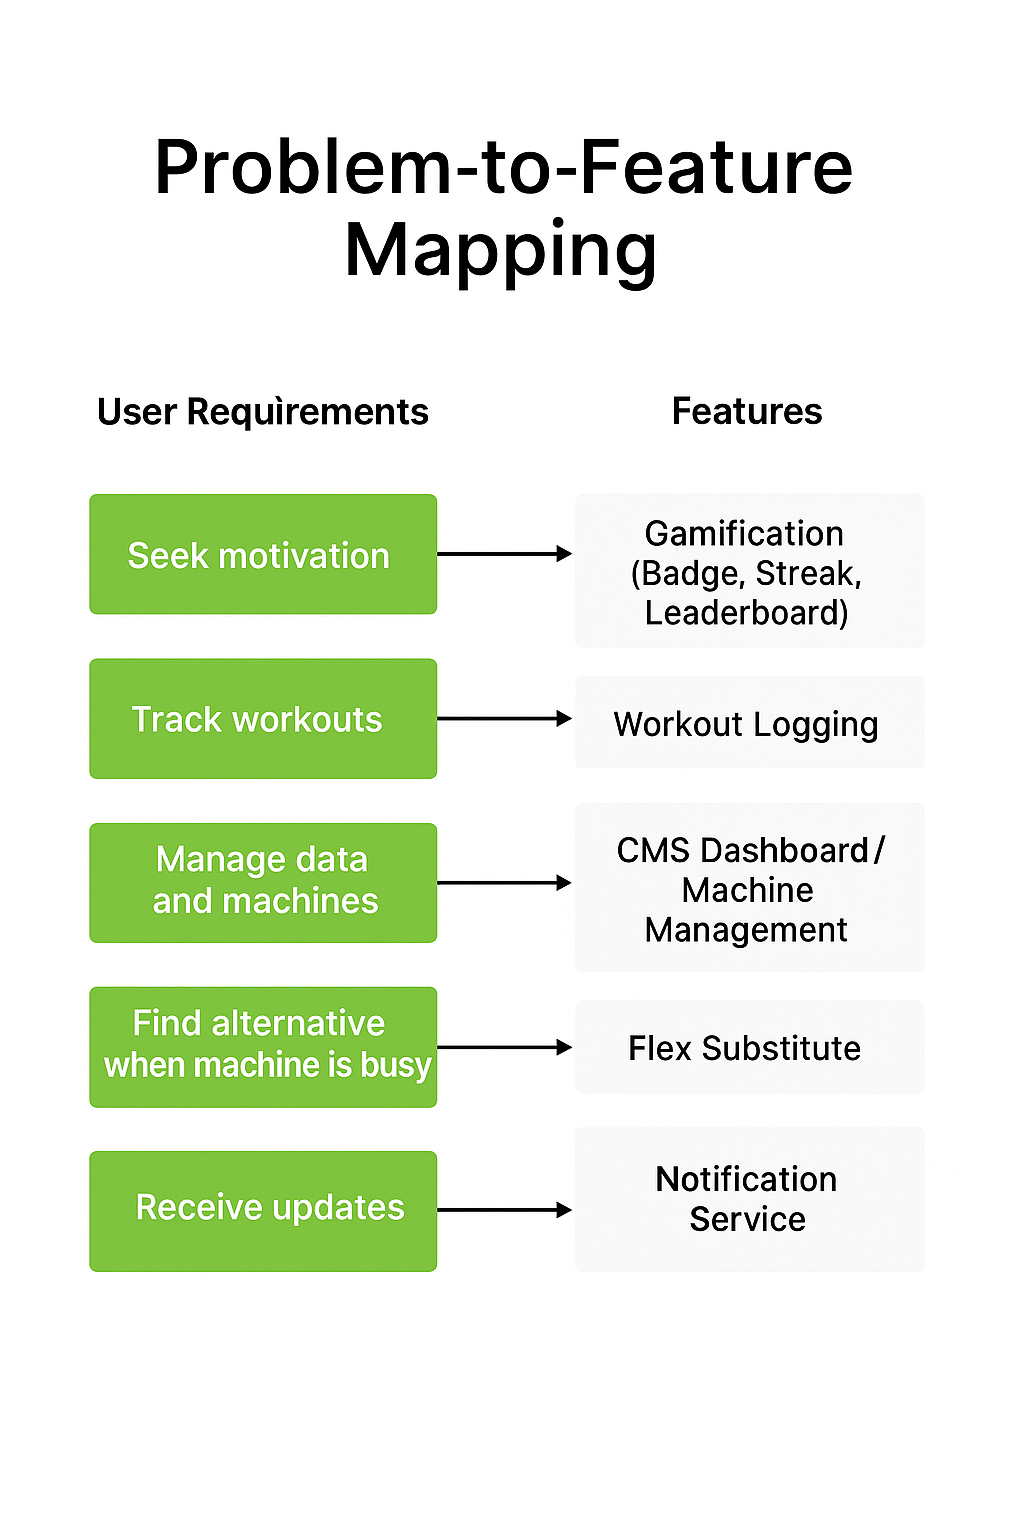
\includegraphics[width=0.35\textwidth]{chapters/Images/Mapping.png}
  \caption{แผนภาพแสดงProblem->Features: กรอบการออกแบบสำหรับ GymMate}
  \label{fig:mapping}
\end{figure}

\subsection{การออกแบบประสบการณ์ผู้ใช้ (User Experience Design)}
\label{subsec:ux-design}

ขั้นตอนการออกแบบประสบการณ์ผู้ใช้ประกอบด้วย:
\begin{itemize}
    \item การกำหนด Use Cases หลัก (Core Use Cases Definition)
    \item การออกแบบ User Flows และเส้นทางผู้ใช้ (User Flows \& Journey Design)
    \item การสร้าง Wireframes และ Prototypes
    \item การทดสอบความใช้งานได้ (Usability Testing)
\end{itemize}
\vspace{1em}

\begin{figure}[h!]
  \centering
  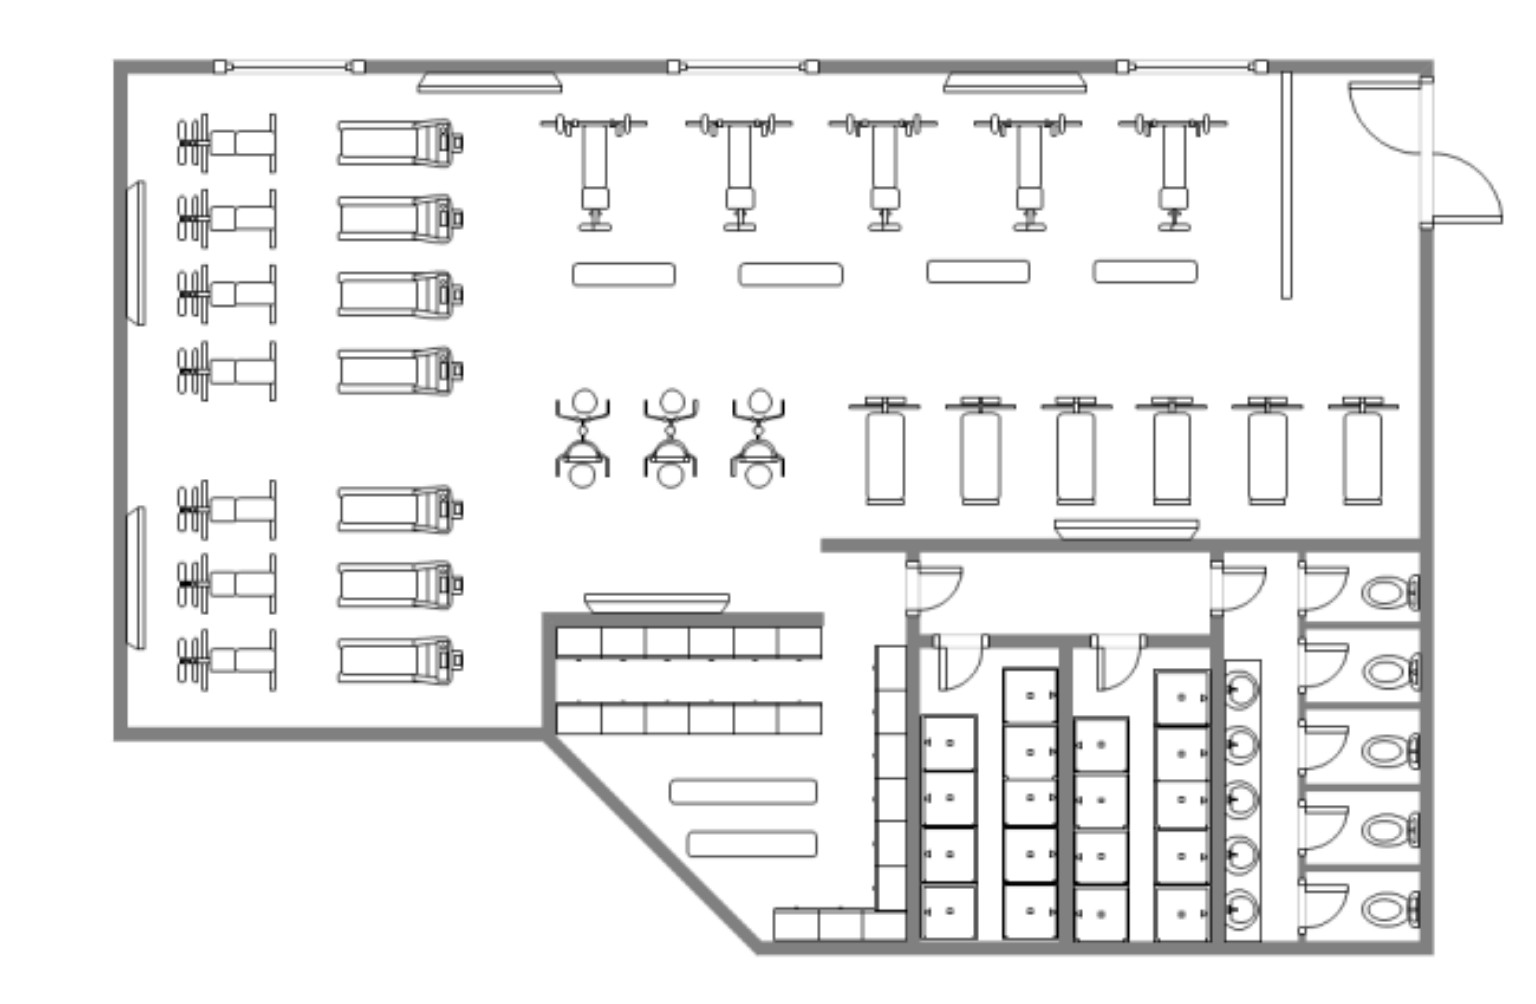
\includegraphics[width=0.35\textwidth]{chapters/Images/Floorplan.png}
  \caption{Simplified Floor Plan of Gym Layout in GymMate}
  \label{fig:floorplan}
\end{figure}

\subsection{การออกแบบระบบและข้อมูล (System \& Data Design)}
\label{subsec:system-design}

การออกแบบด้านเทคนิคของระบบประกอบด้วย:
\begin{itemize}
    \item การออกแบบ Domain Model
    \item การออกแบบโครงสร้างข้อมูล (Data Structure Design)
    \item การออกแบบสถาปัตยกรรมซอฟต์แวร์ (Software Architecture Design)
    \item การออกแบบ API (API Design)
\end{itemize}

\subsection{การออกแบบความปลอดภัยและความเป็นส่วนตัว (Security \& Privacy by Design)}
\label{subsec:security-design}

การออกแบบด้วยแนวคิดความปลอดภัยและความเป็นส่วนตัวตั้งแต่เริ่มต้น:
\begin{itemize}
    \item การวิเคราะห์ความเสี่ยงด้านความปลอดภัย (Security Risk Analysis)
    \item การออกแบบตามหลัก PDPA (PDPA Compliance Design)
    \item การกำหนดนโยบายการเข้าถึงข้อมูล (Data Access Policies)
    \item การป้องกันข้อมูลส่วนบุคคล (Personal Data Protection)
\end{itemize}

\subsection{การออกแบบโครงสร้างพื้นฐานและการส่งมอบ (Infrastructure \& Delivery Design)}
\label{subsec:infrastructure-design}

การออกแบบสภาพแวดล้อมและกระบวนการส่งมอบ:
\begin{itemize}
    \item การออกแบบสถาปัตยกรรมระบบ (System Architecture Design)
    \item การวางแผนโครงสร้างพื้นฐาน (Infrastructure Planning)
    \item การออกแบบ Pipeline CI/CD (CI/CD Pipeline Design)
    \item กลยุทธ์การ deployment (Deployment Strategies)
\end{itemize}

\subsection{การทดสอบและประกันคุณภาพ (Testing \& Quality Assurance)}
\label{subsec:testing-qa}

ขั้นตอนสุดท้ายก่อนการส่งมอบ:
\begin{itemize}
    \item การวางแผนการทดสอบที่ขับเคลื่อนด้วยความปลอดภัย (Security-Driven Test Planning)
    \item การเขียน Test Cases
    \item การทดสอบการแทรกซึมและความปลอดภัย (Penetration \& Security Testing)
    \item การตรวจสอบคุณภาพก่อนส่งมอบ (Pre-Delivery Quality Verification)
\end{itemize}
